\chapter{Validação experimental, Simulação e Testes}
\label{chap:validacao}

\section{Introdução}
\label{validacao:sec:introducao}
Neste capítulo será apresentada a interface fornecida na implementação tal como a sua utilidade tanto
durante o desenvolvimento do projeto como para uma possível prova parcial do bom funcionamento deste.
Irá ser feita uma descrição de como é disposta a informação da rede/sistema, como são representados os
nós, as estruturas de dados distribuídas e do histórico de acontecimentos na rede.
Este histórico será o elemento principal na prova parcial da implementação, pois para o bom funcionamento 
do sistema é necessário que dois tipos de eventos tenham a mesma ordem, estes sendo, as entradas dos \emph{Node} 
na fila principal (que está diretamente ligada ao atual detentor do objeto) têm de seguir a mesma ordem que a chegada do
acesso do objeto aos \emph{Nodes} que o pediram o acesso a este.

\section{Interface de Visualização}
\label{validacao:sec:interface}
Para demonstrar o funcionamento e o estado do sistema, foi desenvolvida uma interface gráfica. Nesta secção serão descritos os componentes apresentados na interface de visualização.

\begin{figure}[!htb]
\centering
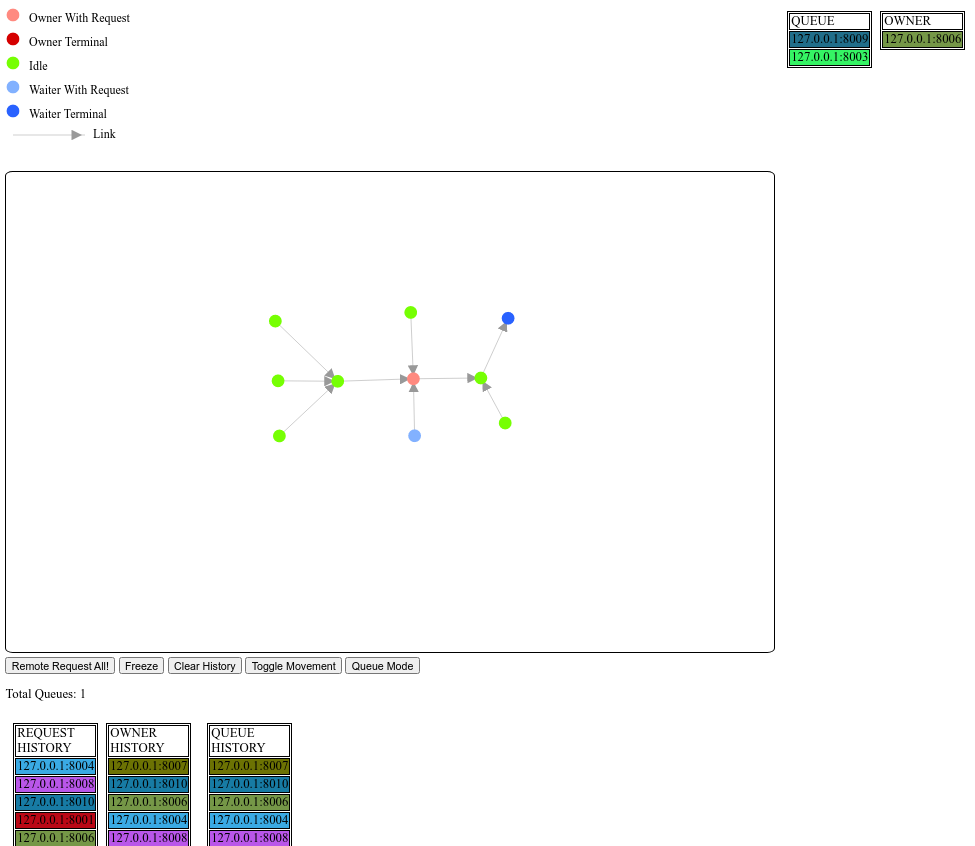
\includegraphics[width=300pt]{relatorio_overview.png}
\caption{Visão geral da interface.}
\end{figure}

Esta interface contém a informação sobre as duas estruturas de dados presentes no sistema, tabelas que contêm o histórico de vários eventos no sistema, e botões para interagir com o sistema e a visualização.

% TODO: Pôr uma introdução aqui.

\subsection*{Representação das Estruturas de Dados}
Na parte central da interface está apresentado um grafo, no qual os círculos representam os \emph{Nodes} e as setas representam os \emph{Links}. 
Também está presente uma etiqueta que indica qual o tipo do \emph{Node} corresponde à cor de um \emph{Node}.
As ligações (\emph{Links}) entre os \emph{Nodes} e as cores dos \emph{Nodes} são atualizadas dependendo do estado conhecido do sistema. 

Ou seja, há uma animação que vai evoluindo conforme o estado da rede conhecido pelo \emph{Node} de visualização, na qual é possível acompanhar que o comportamento de cada \emph{Node} altera a estado do rede.

É possível saber mais informação sobre cada \emph{Node}, deixando o ponteiro do rato por cima de um \emph{Node} e é possível forçar um \emph{Node} a realizar um pedido ao clicar neste.

Existe também o modo de filas/\emph{Queue}, que após pressionar o botão \emph{Queue Mode} (ver subsecção \ref{validacao:subsec:historico}
) as setas entre nós passam a demonstrar as ligações de filas/\emph{Queues} entre os \emph{Nodes}, ao invés das ligações do diretório.

Também estão apresentadas duas tabelas ao lado direito, com os títulos \emph{Queue} e \emph{Owner}, que representam a \emph{Queue} ``Principal'' e o atual \emph{Owner} conhecido.

\subsection*{Históricos}
\label{validacao:subsec:historico}
Na parte inferior da interface estão apresentadas 3 tabelas que contém informação sobre os seguintes históricos:
\begin{description}
    \item [\emph{Request History}] Histórico dos pedidos realizados pelos \emph{Nodes}.
    \item [\emph{Owner History}] Histórico dos \emph{Nodes} que tiveram o acesso ao objeto.
    \item [\emph{Queue History}] Histórico dos \emph{Nodes} da fila principal, isto é, a ordem da futura chegada do objeto aos \emph{Nodes}.
\end{description}

Esta informação não representa o estado da rede, mas é utilizada em testes. No entanto, o seu uso será descrito na secção \ref{validacao:sec:testes}.
% o grafo que representa o grafo distribuído/diretório e uma tabela que representa a fila/lista de espera ``Principal'' (que está diretamente ligada ao atual \emph{Owner}), 

\subsection*{Botões}
Na interface estão disponíveis 5 botões diferentes que permitem a iteração com o sistema e a visualização. A funcionalidade de cada botão é a seguinte:
\begin{description}
    \item [Remote Request All] - Força todos os \emph{Nodes} conhecidos a realizarem pedidos. Usado para testes.
    \item [Freeze] - Para qualquer atualização da interface de visualização.
    \item [Clear History] - Apaga as tabelas de histórico.
    \item [Toggle Movement] - Bloqueia o movimento de todos os círculos que representam os \emph{Nodes} no grafo.
    \item [Queue Mode] - Ativa o modo de demonstração das filas.

\end{description}

Foi disponibilizado um vídeo na plataforma \emph{YouTube}, no qual é possível observar a interface e o seu funcionamento. \url{https://youtu.be/de_02kPA3qc}
\section{Testes}
\label{validacao:sec:testes}
%TODO: explicar o quão diferente é a única implementação conhecida
No desenvolvimento foi necessário testar a implementação e também provar o seu bom funcionamento, no entanto não foi possível fazer-se uso de métodos formais de prova deste sistema, nem de comparar esta implementação com outra existente, visto que, a implementação feita no decorrer deste projeto é muito diferente da única conhecida \cite{aleph}.
						%mudar "histórico VVVVV"
Ainda assim é possível testar o bom funcionamento do sistema fazendo o uso dos elementos presentes na interface gráfica disponibilizada.
% Talvez especificar todas as questões de bom funcionamento?

Nem todos os elementos da visualização estão atualizados em qualquer momento, por exemplo, ambos o grafo e as tabelas da fila ``Principal'' podem estar em desacordo com o estado real do diretório, pois ambos dependem da última informação conhecida pelo \emph{Node} de visualização, que pode ter um \emph{Delay} causado tanto pela atualização (ou \emph{Refresh Rate}) da interface, a rede usada para comunicação, a sincronização da chegada de informação, etc., mas ao longo do decorrer do sistema, estes serão corrigidos.


É possível, na demonstração gráfica do diretório (o grafo) ser mostrado um estado impossível, como, por exemplo, mostrar vários \emph{Owners}, sendo que na realidade só existe um único, ou uma ligação em falta, porém, a implementação estaria errada caso um \emph{Node} se ligar a um \emph{Node} que previamente não era seu vizinho, pois, como definido no protocolo estudado, os vizinhos de um \emph{Node} são sempre as mesmos, apenas as ligações entre estes é que são alteradas (invertidas).

No entanto, o uso mais indicado do grafo e das tabelas da fila e atual \emph{Owner} é de visualização e demonstração de como funciona o sistema/protocolo, e não como prova, devido aos problemas de atualização presentes. 

Para uma evidência mais forte, fez-se uso das 3 tabelas dos históricos. 
Como referido anteriormente, a tabela \emph{Queue History} mostra o histórico dos \emph{Nodes} que entraram na fila ``Principal'', e a passagem do acesso ao objeto tem de seguir a ordem dessa fila, e a ordem por onde circula o objeto é mostrado na tabela \emph{Owner History}, logo, caso as tabelas \emph{Queue History} e \emph{Owner History} demonstrem os \emph{Nodes} com ordens diferentes, o sistema está errado, visto que o objeto não ``seguiu'' a ordem esperada.

A tabela \emph{Request History} demonstra que a ordem pela qual os \emph{Nodes} realizam pedidos ou que a ordem
que \emph{Node} de visualização recebe a atualização de que esses \emph{Nodes} realizaram pedidos pode ser diferente da ordem na fila ``Principal''.
Esta pode ser apresentada com uma ordem dos \emph{Nodes} diferente à apresentada nas outras tabelas, visto que, caso um \emph{Node} realize um pedido, este pedido pode demorar mais tempo a chegar a um \emph{Node Terminal} do que, por exemplo, um \emph{Node} que realize mais tarde um pedido e que esteja diretamente ligado ao \emph{Node Terminal}.

É possível observar este fenómeno quando há \emph{Nodes} muito distantes de um \emph{Waiter Terminal} ou quando há um grande número de pedidos a circular na rede,
que pode ser demonstrado usando o botão ``Request All'' disponível na interface.

Foi gravado um vídeo, o qual se enconta disponível na plataforma \emph{YouTube}, no qual é feita uma comparação das várias tabelas. \url{https://youtu.be/FIdTcE4UJsg}


\section{Conclusões}
\label{validacao:sec:conclusoes}
Neste capítulo foi esclarecida a representação dos vários elementos do sistema, em que se dispõe um
grafo para representar as várias ligações entre os nós, quer estas sejam ligações do diretório ou das filas, 
uma tabela que contém os endereços dos \emph{Nodes} que estão presentes na fila ``Principal''.
Foram apresentados os usos do botão, estes que servem para a interação com a interface ou até mesmo com o sistema.
A secção de maior interesse para este projeto é a secção de Testes, pois, recorreu-se ao uso do histórico dos eventos para 
se provar parcialmente o bom funcionamento da implementação conseguida no projeto, em que, para que o sistema não apresente falhas
é necessário que a ordem de ``chegada'' dos \emph{Nodes} à fila ``Principal'' (esta é a fila que tem o atual \emph{Owner} como cabeça de fila)
seja a mesma que os \emph{Nodes} recebem o acesso ao objeto.
